\hypertarget{interface_s_s_y_labelled_list}{
\section{SSYLabelledList Class Reference}
\label{interface_s_s_y_labelled_list}\index{SSYLabelledList@{SSYLabelledList}}
}
This class provides a control which consists of a non-editable NSTextField {\em label\/} and, below it, a non-editable list of strings (choices), displayed in an NSScrollView+NSTableView. The height of the scroll/table is adjusted to fit the content, up to a given maximum table height.  


{\tt \#import $<$SSYLabelledList.h$>$}

Inheritance diagram for SSYLabelledList::\begin{figure}[H]
\begin{center}
\leavevmode
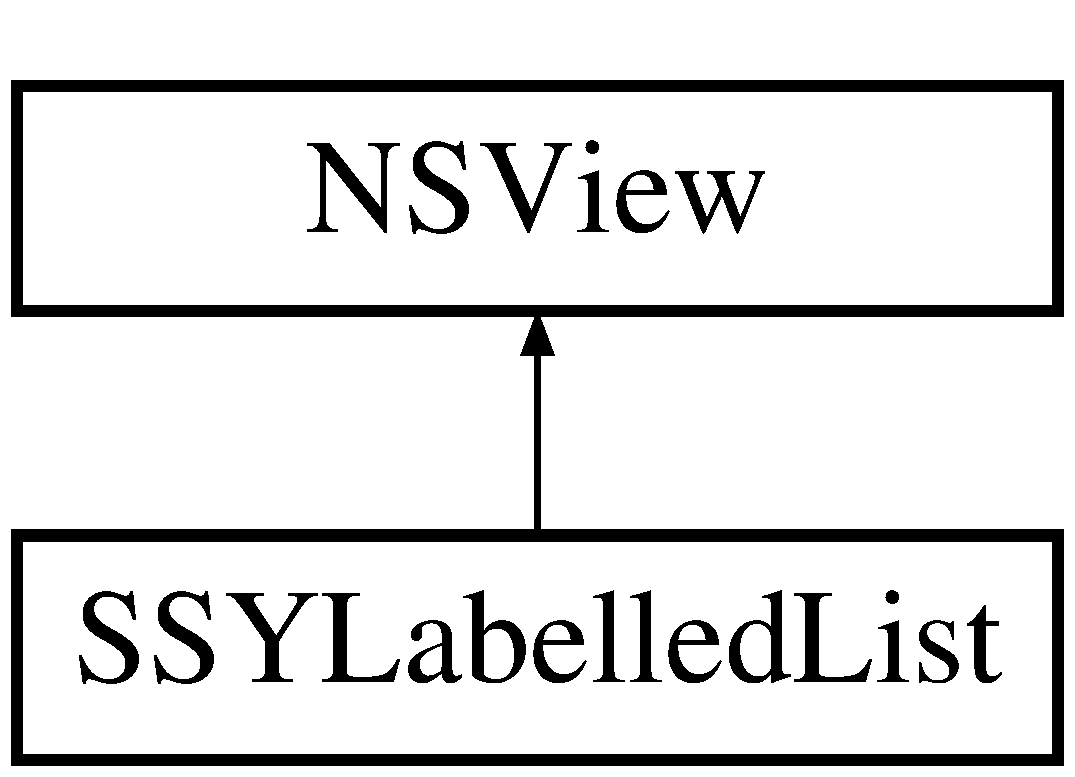
\includegraphics[height=2cm]{interface_s_s_y_labelled_list}
\end{center}
\end{figure}
\subsection*{Public Member Functions}
\begin{CompactItemize}
\item 
\hypertarget{interface_s_s_y_labelled_list_f55eba1cf5bd693dc76dd8fdb8c4e092}{
(NSIndexSet $\ast$) - \hyperlink{interface_s_s_y_labelled_list_f55eba1cf5bd693dc76dd8fdb8c4e092}{selectedIndexes}}
\label{interface_s_s_y_labelled_list_f55eba1cf5bd693dc76dd8fdb8c4e092}

\begin{CompactList}\small\item\em Returns the set of indexes selected in the receiver's list, from the receiver's choices. \item\end{CompactList}\item 
\hypertarget{interface_s_s_y_labelled_list_252f3b62f2a9f8fd5ddcfb728076a6d3}{
(NSArray $\ast$) - \hyperlink{interface_s_s_y_labelled_list_252f3b62f2a9f8fd5ddcfb728076a6d3}{selectedValues}}
\label{interface_s_s_y_labelled_list_252f3b62f2a9f8fd5ddcfb728076a6d3}

\begin{CompactList}\small\item\em Returns the set of strings selected in the receiver's list. \item\end{CompactList}\item 
(void) - \hyperlink{interface_s_s_y_labelled_list_db8c7701fa1bab293368423691e60a61}{setAllowsMultipleSelection:}
\begin{CompactList}\small\item\em Sets whether or not the receiver's table view allows a multiple selection. \item\end{CompactList}\item 
\hypertarget{interface_s_s_y_labelled_list_aee783c884612f2d46e67d15fba43f42}{
(void) - \hyperlink{interface_s_s_y_labelled_list_aee783c884612f2d46e67d15fba43f42}{setSelectedIndexes:}}
\label{interface_s_s_y_labelled_list_aee783c884612f2d46e67d15fba43f42}

\begin{CompactList}\small\item\em Sets the set of indexes to be initially selected (suggested) when the list is displayed. \item\end{CompactList}\end{CompactItemize}
\subsection*{Static Public Member Functions}
\begin{CompactItemize}
\item 
(\hyperlink{interface_s_s_y_labelled_list}{SSYLabelledList} $\ast$) + \hyperlink{interface_s_s_y_labelled_list_2a5643a553c82edcf83ec234f21923e7}{listWithLabel:choices:maxTableHeight:}
\begin{CompactList}\small\item\em Convenience method for getting an autoreleased instance of this class. \item\end{CompactList}\end{CompactItemize}
\subsection*{Protected Attributes}
\begin{CompactItemize}
\item 
\hypertarget{interface_s_s_y_labelled_list_7d76a6e19adfd33987f653c6ec754fbb}{
NSArray $\ast$ \textbf{choices}}
\label{interface_s_s_y_labelled_list_7d76a6e19adfd33987f653c6ec754fbb}

\item 
\hypertarget{interface_s_s_y_labelled_list_1072969e548c452b1d9083a23546863a}{
NSTextField $\ast$ \textbf{labelView}}
\label{interface_s_s_y_labelled_list_1072969e548c452b1d9083a23546863a}

\item 
\hypertarget{interface_s_s_y_labelled_list_3d47c5c985b2d6be299be3418c71004a}{
NSScrollView $\ast$ \textbf{scrollView}}
\label{interface_s_s_y_labelled_list_3d47c5c985b2d6be299be3418c71004a}

\end{CompactItemize}


\subsection{Detailed Description}
This class provides a control which consists of a non-editable NSTextField {\em label\/} and, below it, a non-editable list of strings (choices), displayed in an NSScrollView+NSTableView. The height of the scroll/table is adjusted to fit the content, up to a given maximum table height. 

May be used, for example for a user to select several items from a list. 

\subsection{Member Function Documentation}
\hypertarget{interface_s_s_y_labelled_list_2a5643a553c82edcf83ec234f21923e7}{
\index{SSYLabelledList@{SSYLabelledList}!listWithLabel:choices:maxTableHeight:@{listWithLabel:choices:maxTableHeight:}}
\index{listWithLabel:choices:maxTableHeight:@{listWithLabel:choices:maxTableHeight:}!SSYLabelledList@{SSYLabelledList}}
\subsubsection[{listWithLabel:choices:maxTableHeight:}]{\setlength{\rightskip}{0pt plus 5cm}+ ({\bf SSYLabelledList} $\ast$) listWithLabel: (NSString$\ast$) {\em label}\/ choices: (NSArray$\ast$) {\em choices}\/ maxTableHeight: (float) {\em maxTableHeight}}}
\label{interface_s_s_y_labelled_list_2a5643a553c82edcf83ec234f21923e7}


Convenience method for getting an autoreleased instance of this class. 

\begin{Desc}
\item[Parameters:]
\begin{description}
\item[{\em label}]The string in the {\em label\/} which will appear above the list in the returned instance.~ In most cases, append a localized version of \char`\"{}Hold down the 'shift' or $\backslash$xe2$\backslash$x8c$\backslash$x98 key to select more than one.\char`\"{} (Or instead of  escapes, use C format specifier with substution 0x2318.) \item[{\em choices}]An array of strings, to appear in the list \item[{\em maxTableHeight}]The maximum height allowed of the scroll/table view. \end{description}
\end{Desc}
\begin{Desc}
\item[Returns:]The instance, autoreleased \end{Desc}
\hypertarget{interface_s_s_y_labelled_list_db8c7701fa1bab293368423691e60a61}{
\index{SSYLabelledList@{SSYLabelledList}!setAllowsMultipleSelection:@{setAllowsMultipleSelection:}}
\index{setAllowsMultipleSelection:@{setAllowsMultipleSelection:}!SSYLabelledList@{SSYLabelledList}}
\subsubsection[{setAllowsMultipleSelection:}]{\setlength{\rightskip}{0pt plus 5cm}- (void) setAllowsMultipleSelection: (BOOL) {\em flag}}}
\label{interface_s_s_y_labelled_list_db8c7701fa1bab293368423691e60a61}


Sets whether or not the receiver's table view allows a multiple selection. 

If not set, defaults to YES. 

The documentation for this class was generated from the following files:\begin{CompactItemize}
\item 
Documents/Programming/Projects/SSYAlert/Ex-Project-Classes/SSYLabelledList.h\item 
Documents/Programming/Projects/SSYAlert/Ex-Project-Classes/SSYLabelledList.m\end{CompactItemize}
